\section{Variabili del sistema}

\subsection{Forze}
\subsubsection{Forza Peso}
La forza peso è ben definita nel sistema di riferimento $NED$, in quanto è allineata con l'asse $\hat{z}_{NED}$. Può essere trasformata nel sistema di riferimento $FRD$ tramite la matrice di rotazione definita in \eqref{eq:NEDtoFRD}:
\begin{equation}
    \label{eq:Fpeso}
    \left(\vec{F}_P(t)\right)_{FRD} = C_{NED \rightarrow FRD}\begin{bmatrix}
        0 \\
        0 \\
        mg
    \end{bmatrix}_{NED} = \begin{bmatrix}
        -mg\sin\theta (t)          \\
        mg\sin\phi(t)\cos\theta(t) \\
        mg\cos\phi(t)\cos\theta(t)
    \end{bmatrix}_{FRD}
\end{equation}

\begin{note}
    Nella formula $m$ e $g$ sono delle costanti che rappresentano rispettivamente la massa del velivolo e l'accelerazione di gravità.
\end{note}

\subsubsection{Forza Propulsiva}
La forza propulsiva è definita nel sistema di riferimento FRD, in generale non è allineata all'asse $\hat{x}_{FRD}$, ma può essere scomposta in due componenti:

\begin{equation}
    \label{eq:Fpropulsiva}
    \left(\vec{F}_T(t)\right)_{FRD} = \begin{bmatrix}
        T(t) \cos\epsilon \\
        0                 \\
        -T(t) \sin\epsilon
    \end{bmatrix}_{FRD}
\end{equation}

\begin{figure}[H]
    \centering
    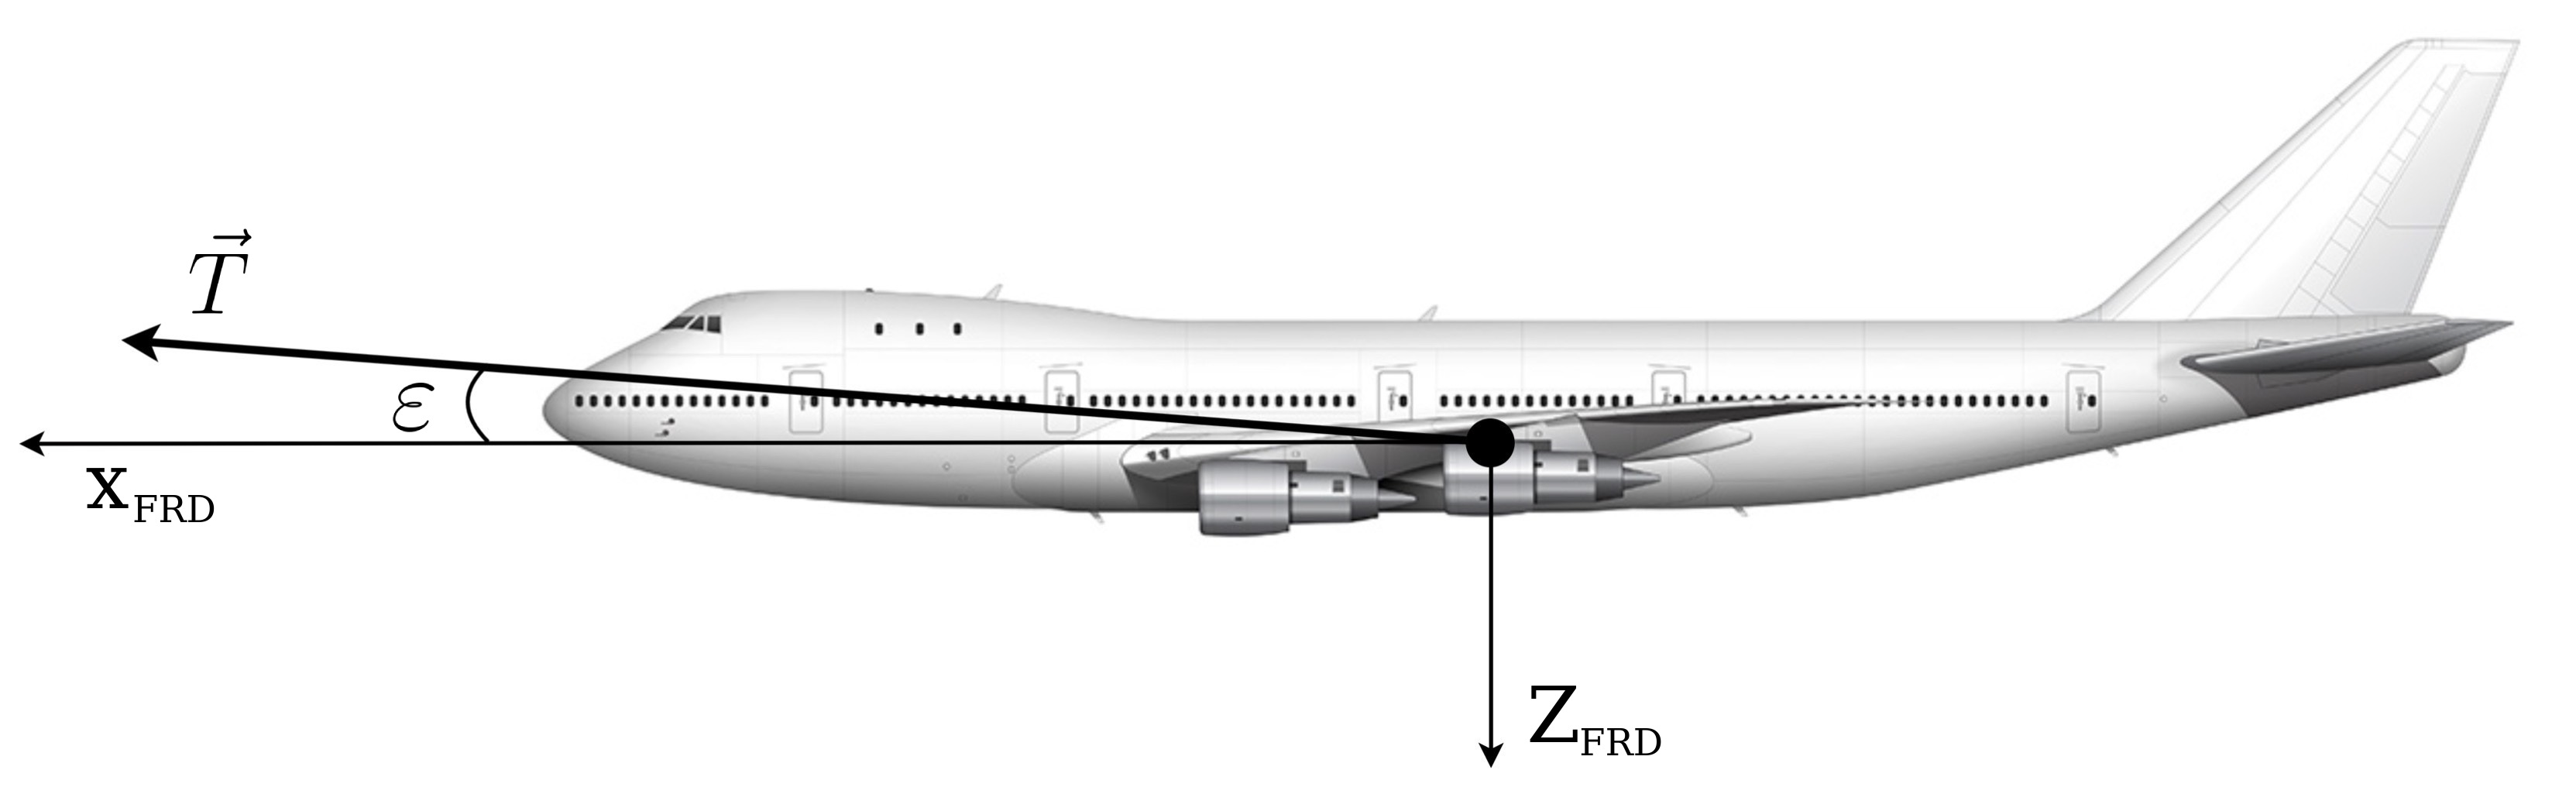
\includegraphics[width=0.7\linewidth]{Immagini/forza_propulsiva.jpg}
    \caption{Vettore $\vec{T}(t)$ e il suo angolo $\epsilon$}
\end{figure}

\begin{note}
    Nella formula $\epsilon$ è una costante determinata dalla struttura del velivolo che rappresenta l'angolo tra il vettore $\vec{T}$ e l'asse $\hat{x}_{FRD}$
\end{note}

\subsubsection{Forze Aerodinamiche}
Le forze aerodinamiche sono ben definite nel sistema di riferimento assi di stabilità.
\begin{equation*}
    \left(\vec{F}_A(t)\right)_{S} = \begin{bmatrix}
        -F_{A_x}(t) \\
        F_{A_y}(t)  \\
        -F_{A_z}(t)
    \end{bmatrix}_{S}
\end{equation*}

In questo caso $F_{A_z}(t)$ rappresenta la portanza, normale al flusso d'aria, mentre $F_{A_x}(t)$ la resistenza aerodinamica, opposta al flusso d'aria.

$F_{A_y}(t)$ è la componente laterale della forza, dovuta all'angolo di derapata $\beta(t)$.

Si possono esprimere le forze aerodinamiche nel sistema di riferimento $FRD$ tramite la matrice di rotazione definita in \eqref{eq:StoFRD}:
\begin{equation}
    \label{eq:Faerodinamica}
    \left(\vec{F}_A(t)\right)_{FRD} = C_{S \rightarrow FRD}\left(\vec{F}_A(t)\right)_{S} = \begin{bmatrix}
        -F_{A_x}(t) \cos\alpha(t) + F_{A_z}(t) \sin\alpha(t) \\
        F_{A_y}(t)                                           \\
        -F_{A_x}(t)\sin\alpha(t) - F_{A_z}(t)\cos\alpha(t)
    \end{bmatrix}_{FRD}
\end{equation}

\begin{note}
    $F_{A_x}(t), F_{A_y}(t), F_{A_z}(t)$ sono funzioni non lineari di altre variabili del sistema. Questa dipendenza verrà analizzata in maggior dettaglio nella sezione \ref{sec:derivateStabilita}.
\end{note}
\subsection{Velocità Angolare}

Diremo $\vec{w}_{FRD}$ la velocità angolare del sistema di riferimento $FRD$ rispetto al sistema inerziale $NED$.

Il sistema $FRD$ è stato definito a partire dal sistema $NED$ come una serie di tre rotazioni i cui angoli sono detti angoli di Eulero \ref{subsec:Eulero}.
Tuttavia la loro derivata non fornisce $\vec{w}_{FRD}$ in quanto i tre angoli non sono descritti nello stesso sistema di riferimento è quindi necessario applicare delle rotazioni:

\begin{equation}
    \label{eq:EulerotoVelocitaAngolare}
    \begin{split}
        \vec{w}_{FRD}(t) & = \begin{bmatrix}
                                 p(t) \\
                                 q(t) \\
                                 r(t)
                             \end{bmatrix} = R_{x}(\phi)R_{y}(\theta) \begin{bmatrix}
                                                                          0 \\
                                                                          0 \\
                                                                          \dot{\psi}(t)
                                                                      \end{bmatrix} + R_{x}(\phi) \begin{bmatrix}
                                                                                                      0               \\
                                                                                                      \dot{\theta}(t) \\
                                                                                                      0
                                                                                                  \end{bmatrix} + I_3 \begin{bmatrix}
                                                                                                                          \dot{\phi}(t) \\
                                                                                                                          0             \\
                                                                                                                          0
                                                                                                                      \end{bmatrix} =
        \\ & = \begin{bmatrix}
            1 & 0            & -\sin\theta(t)           \\
            0 & \cos\phi(t)  & \sin\phi(t)\cos\theta(t) \\
            0 & -\sin\phi(t) & \cos\phi(t)\cos\theta(t)
        \end{bmatrix}\begin{bmatrix}
            \dot{\phi}(t)   \\
            \dot{\theta}(t) \\
            \dot{\psi}(t)
        \end{bmatrix}
    \end{split}
\end{equation}

\subsection{Velocità}
La velocità del velivolo è la velocità del sistema di riferimento $FRD$ rispetto al sistema inerziale $NED$.

\begin{equation}
    \label{eq:velocitaFRD}
    \vec{V}_{FRD}(t) = \begin{bmatrix}
        u(t) \\
        v(t) \\
        w(t)
    \end{bmatrix}_{FRD}
\end{equation}

\subsubsection{Velocità nel Sistema Assi Vento}
Una rappresentazione più naturale del vettore velocità è nel sistema di riferimento assi vento, in quanto è parallelo a $\hat{x}_{W}$.
È poi possibile cambiare il sistema di riferimento ottenendo così una rappresentazione polare della velocità nel sistema $FRD$:

\begin{equation}
    \label{eq:velocitaWind}
    \vec{V}_{FRD}(t) = \begin{bmatrix}
        u(t) \\
        v(t) \\
        w(t)
    \end{bmatrix}_{FRD} = C_{W \rightarrow FRD}\begin{bmatrix}
        |\vec{V}_{FRD}(t)| \\
        0                  \\
        0
    \end{bmatrix}_{W} = |\vec{V}_{FRD}(t)|\begin{bmatrix}
        \cos\alpha(t)\cos\beta(t) \\
        \sin\beta(t)              \\
        \sin\alpha(t)\cos\beta(t)
    \end{bmatrix}
\end{equation}

\begin{figure}[H]
    \centering
    \includegraphics[width=0.4\linewidth]{Immagini/velocità_assi_vento.jpg}
    \caption{Vettore $\vec{V}_{FRD}$ e i suoi angoli $\alpha(t)$ e $\beta(t)$}
\end{figure}

\subsubsection{Velocità nel Sistema NED}
Un'altra rappresentazione utile della velocità è nel sistema di riferimento $NED$, dove può essere espressa come:
\begin{multline}
    \label{eq:velocitaNED}
    \vec{V}_{NED}(t) = \begin{bmatrix}
        \dot{x}(t) \\
        \dot{y}(t) \\
        \dot{z}(t)
    \end{bmatrix}_{NED} = C_{FRD \rightarrow NED}\begin{bmatrix}
        u(t) \\
        v(t) \\
        w(t)
    \end{bmatrix}_{FRD} = \\ = \begin{bmatrix}
        \cos\theta\cos\psi \: u + \left(\sin\phi\sin\theta\cos\psi + \cos\phi\sin\psi\right)v + \left(\cos\phi\sin\theta\cos\psi - \sin\phi\sin\psi\right)w \\
        \cos\theta\sin\psi \: u + \left(\sin\phi\sin\theta\sin\psi - \cos\phi\cos\psi\right)v + \left(\cos\phi\sin\theta\sin\psi + \sin\phi\cos\psi\right)w \\
        -\sin\theta \: u + \sin\phi\cos\theta \: v + \cos\phi\cos\theta \: w
    \end{bmatrix}
\end{multline}

\textbf{Nota:} \textit{Per semplicità di lettura è omessa la dipendenza dal tempo di $\theta$, $\phi$, $\psi$, $u$, $v$, $w$}

\subsection{Accelerazione}

Affinché siano valide le equazioni cardinali è necessario applicarle su un sistema di riferimento inerziale, per questo motivo è necessario calcolare $\vec{a}_{NED}$.
Per farlo si sfrutta la relazione di Poisson, $\frac{d}{dt}\vec{u}(t) = \vec{w}_{FRD}(t) \times \vec{u}(t)$, la cui dimostrazione è illustrata in \cite{zotto_fisica1}

\begin{figure}[H]
    \centering
    \begin{tikzpicture}
        \draw[->] (-3,0)--(3,0) node[right]{$x$};
        \draw[->] (0,-1)--(0,3) node[above]{$y$};
        \draw[line width=2pt,blue,-stealth](0,2)--(-0.65,2) node[left]{$\frac{d}{dt}\vec{u}(t)$};
        \draw[line width=2pt,-stealth](0,0)--(0, 2) node[right]{$\vec{u}(t)$};
        \draw[thick,orange] (0,0) circle (0.25);
        \fill[orange] (0,0) circle (2pt);
        \node[orange, anchor=south west] at (0.22, 0.22) {$\vec{w}_{FRD}(t)$};
        \draw[thick,->, orange] (0,1) arc[start angle=90,end angle=120,radius=1.2];
    \end{tikzpicture}
    \caption{Intuizione grafica alla relazione di Poisson}
\end{figure}

\begin{equation}
    \label{eq:accelerazioneNED}
    \begin{split}
        \vec{a}_{NED}(t) & = \left(\frac{d}{d t}\vec{V}_{FRD}(t)\right)_{NED} = \sum_{i=x,y,z} \frac{d}{d t}\left(V_i(t)\vec{u}_i(t)\right) = \\
                         & = \sum_{i=x,y,z} a_i(t)\vec{u}_i(t) + V_i(t)\left(\vec{w}_{FRD}(t)\times\vec{u}_i(t)\right) =                      \\
                         & = \left(\frac{d}{d t} \vec{V}_{FRD}(t)\right)_{FRD} + \vec{w}_{FRD}(t)\times\vec{V}_{FRD}(t) =                     \\
                         & = \begin{bmatrix}
                                 \dot{u}(t) \\
                                 \dot{v}(t) \\
                                 \dot{w}(t)
                             \end{bmatrix} + \begin{bmatrix}
                                                 p(t) \\
                                                 q(t) \\
                                                 r(t)
                                             \end{bmatrix}\times \begin{bmatrix}
                                                                     u(t) \\
                                                                     v(t) \\
                                                                     w(t)
                                                                 \end{bmatrix}
        = \begin{bmatrix}
              \dot{u} + \left(qw - rv\right) \\
              \dot{v} + \left(ru - pw\right) \\
              \dot{w} + \left(pv - qu\right)
          \end{bmatrix}
    \end{split}
\end{equation}

\textbf{Nota:} \textit{Per semplicità di lettura è omessa la dipendenza dal tempo di u, v, w, p, q, r (e derivate).}

\subsection{Momento Angolare}
Il momento angolare di una massa infinitesimale $dm$ appartenente al velivolo è definito come:
\begin{equation*}
    d\vec{H}_{dm}(t) = \vec{r}_{dm}\times \left(\vec{V}_{dm}(t)\right)_{NED} dm
\end{equation*}

Dove $\vec{r}_{dm}$ è la posizione della massa $dm$ rispetto al centro di massa dell'aereomobile.

\begin{figure}[H]
    \centering
    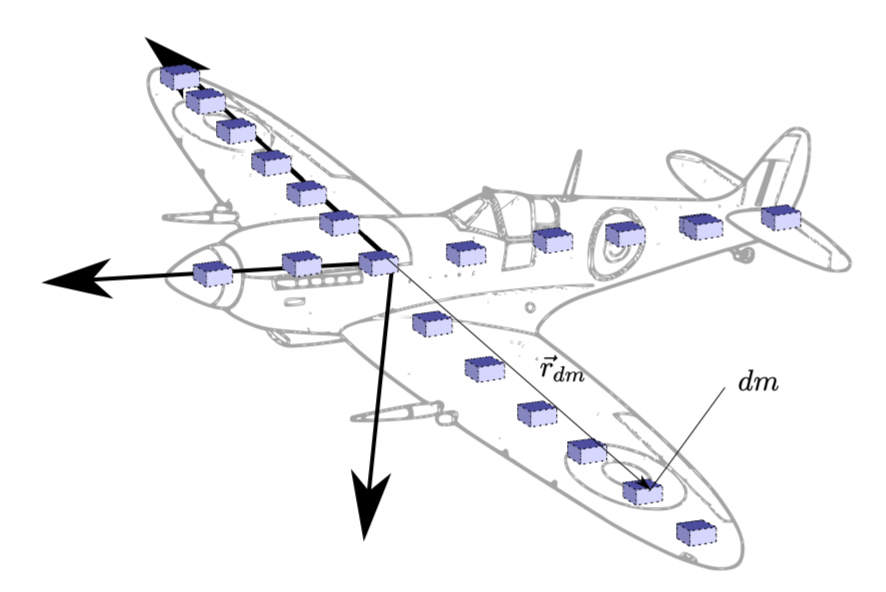
\includegraphics[width=0.5\linewidth]{Immagini/momento_angolare.jpg}
    \caption{Aeromobile descritto da masse infinitesimali \cite{smith_aircraft_flight_mechanics}}
\end{figure}

\subsubsection{Velocità Assoluta}
La velocità assoluta, nel sistema di riferimento inerziale viene calcolata in modo simile a quanto fatto per l'accelerazione:

\begin{equation*}
    \begin{split}
        \left(\vec{V}_{dm}(t)\right)_{NED} & = \left(\frac{d}{d t}\vec{r}_{dm}\right)_{NED} = \left(\frac{d}{d t}\vec{r}_{dm}\right)_{FRD} + \vec{w}_{FRD}(t) \times \vec{r}_{dm} = \\ &= \vec{w}_{FRD}(t) \times \vec{r}_{dm} = \begin{bmatrix}
            q(t)z_{dm} - r(t)y_{dm} \\
            r(t)x_{dm} - p(t)z_{dm} \\
            p(t)y_{dm} - q(t)x_{dm}
        \end{bmatrix}
    \end{split}
\end{equation*}

\begin{note}
    Qui si assume che $\vec{r}_{dm}$ sia costante nel tempo, si sta quindi assumendo che il velivolo sia un corpo rigido, ovvero con flessioni della struttura trascurabili.
\end{note}

\subsubsection{Momento Angolare Infinitesimo}
Il momento angolare di una massa infinitesimale $dm$ è quindi:

\begin{equation*}
    d\vec{H}_{dm}(t) = \vec{r}_{dm}\times \left(\vec{V}_{dm}(t)\right)_{NED} dm = \begin{bmatrix}
        p(t)\left(y_{dm}^2 + z_{dm}^2\right) - q(t)\:x_{dm}y_{dm} - r(t)\:x_{dm}z_{dm} \\
        q(t)\left(x_{dm}^2 + z_{dm}^2\right) - r(t)\:y_{dm}z_{dm} - p(t)\:x_{dm}y_{dm} \\
        r(t)\left(x_{dm}^2 + y_{dm}^2\right) - p(t)\:x_{dm}z_{dm} - q(t)\:y_{dm}z_{dm}
    \end{bmatrix} dm
\end{equation*}

\subsubsection{Momento Angolare Totale}
Il momento angolare totale è l'integrale del momento angolare infinitesimo sul volume dell'aeromobile:

\begin{align*}
    \vec{H}(t) & = \int_{V} d\vec{H}_{dm}(t) dm = \\ &= \begin{bmatrix}
        p(t)\int_V\left(y_{dm}^2 + z_{dm}^2\right) dm - q(t)\int_Vx_{dm}y_{dm}dm - r(t)\int_Vx_{dm}z_{dm}dm \\
        q(t)\int_V\left(x_{dm}^2 + z_{dm}^2\right) dm - r(t)\int_Vy_{dm}z_{dm}dm - p(t)\int_Vx_{dm}y_{dm}dm \\
        r(t)\int_V\left(x_{dm}^2 + y_{dm}^2\right) dm - p(t)\int_Vx_{dm}z_{dm}dm - q(t)\int_Vy_{dm}z_{dm}dm
    \end{bmatrix}
\end{align*}

Gli integrali così ottenuti sono definiti come i momenti e i prodotti di inerzia del velivolo \cite{smith_aircraft_flight_mechanics}:
\begin{equation*}
    \begin{split}
        I_{xx} = \int_V \left(y_{dm}^2 + z_{dm}^2\right) dm \\
        I_{yy} = \int_V \left(x_{dm}^2 + z_{dm}^2\right) dm \\
        I_{zz} = \int_V \left(x_{dm}^2 + y_{dm}^2\right) dm \\
        I_{xy} = I_{yx} = \int_V x_{dm}y_{dm} dm            \\
        I_{xz} = I_{zx} = \int_V x_{dm}z_{dm} dm            \\
        I_{yz} = I_{yz} = \int_V y_{dm}z_{dm} dm
    \end{split}
\end{equation*}

Sostituendo questi integrali nella definizione di $\vec{H}$ si ottiene:

\begin{equation*}
    \vec{H}(t) = \begin{bmatrix}
        I_{xx}p(t) - I_{xy}q(t) - I_{xz}r(t) \\
        I_{yy}q(t) - I_{yz}r(t) - I_{xy}p(t) \\
        I_{zz}r(t) - I_{xz}p(t) - I_{yz}q(t)
    \end{bmatrix} = \begin{bmatrix}
        I_{xx}   & - I_{xy} & - I_{xz} \\
        - I_{yx} & I_{yy}   & - I_{yz} \\
        - I_{xz} & - I_{zy} & I_{zz}
    \end{bmatrix} \vec{w}_{FRD}(t) = I \vec{w}_{FRD}(t)
\end{equation*}

\begin{note}
    $I$ è definito come il \textbf{tensore di inerzia}.
\end{note}

Nel caso del Boeing 747 il velivolo è simmetrico lungo il suo asse longitudinale, quindi $I_{xy}=I_{yx}=I_{yz}=I_{zy}=0$:
\begin{equation}
    \label{eq:TensoreInerzia}
    I = \begin{bmatrix}
        I_{xx}   & 0      & - I_{xz} \\
        0        & I_{yy} & 0        \\
        - I_{zx} & 0      & I_{zz}
    \end{bmatrix}
\end{equation}

\subsubsection{Momento Angolare}
Il momento angolare è quindi definito come:
\begin{equation}
    \label{eq:momentoAngolare}
    \vec{H}(t) = I \vec{w}_{FRD}(t) = \begin{bmatrix}
        I_{xx}p(t) - I_{xz}r(t) \\
        I_{yy}q(t)              \\
        - I_{xz}p(t) + I_{zz}r(t)
    \end{bmatrix}
\end{equation}
